\documentclass[11pt,a4paper]{article}

\usepackage[margin=2.3cm]{geometry}
\usepackage{graphicx}
\usepackage{amsmath}
\usepackage{amssymb}
\usepackage{siunitx}
\usepackage{booktabs}
\usepackage{caption}
\usepackage{subcaption}
\usepackage{hyperref}
\usepackage{float}
\usepackage{xcolor}
\usepackage{listings}
\usepackage{array}
\usepackage{longtable}

\sisetup{
  detect-all,
  separate-uncertainty=true,
  per-mode=symbol
}

\hypersetup{
  colorlinks=true,
  linkcolor=blue!55!black,
  citecolor=blue!55!black,
  urlcolor=blue!55!black,
  pdftitle={Integrated Photonics Design of an SOI Microring Resonator Sensor},
  pdfauthor={Lucas Wang and Group Members}
}

\lstset{
  basicstyle=\ttfamily\small,
  breaklines=true,
  frame=single,
  columns=fullflexible
}

\title{\textbf{Integrated Photonics Design of an SOI Microring Resonator Sensor}\\
\large ELEC5516 Electrical and Optical Sensor Design\\
Lab 5: Integrated Photonics Design - Microring Resonator}
\author{Lucas Wang and Group Members\\
School of Electrical and Computer Engineering\\
The University of Sydney}
\date{May 2026}

\begin{document}
\maketitle

\begin{abstract}
This report documents the design workflow for an SOI add-drop microring resonator sensor near \SI{1550}{\nano\metre}. The intended waveguide cross-section is \SI{400}{\nano\metre} by \SI{200}{\nano\metre}, with design targets of \SI{26.2}{\nano\metre} free spectral range (FSR), drop-port quality factor near 1800, and drop-port finesse near 26. The report combines the ELEC5516 lab procedure with Lecture 12 sensor interrogation principles, and describes the intended multi-level simulation route using Ansys Lumerical INTERCONNECT, MODE/FDE, and varFDTD. No exported simulation spectra, mode tables, monitor data, or gap sweep CSV/JSON files were present at generation time. Consequently, measured FSR, resonance wavelength, linewidth, quality factor, finesse, modal indices, coupling length, and varFDTD verification values are marked as TODO rather than fabricated. Target-based calculations are included only where they follow directly from the stated design targets and equations.
\end{abstract}

\tableofcontents
\newpage

\section{Introduction}
Integrated photonic sensors exploit guided optical fields whose phase, amplitude, or resonance spectrum changes when a physical or chemical measurand perturbs the optical path. A microring resonator is especially attractive because a compact ring stores optical energy over many round trips, converting small effective-index changes into measurable resonance wavelength shifts.

The design platform considered in this laboratory is silicon-on-insulator (SOI). SOI is suitable for integrated photonic sensing because it is compatible with mature CMOS-style fabrication, provides high refractive-index contrast between silicon and silicon dioxide, supports strong optical confinement, and enables compact photonic circuits. In a sensor implementation, external refractive index, temperature, strain, or biochemical binding can change the guided effective index \(n_{\mathrm{eff}}\) or the round-trip optical path length. The resonance wavelength then shifts, enabling the measurand to be inferred from spectral or intensity interrogation.

The laboratory notes define an open-ended design task in which the ring is first modelled at circuit level in INTERCONNECT and then refined using MODE/FDE and varFDTD \cite{labmanual}. This report follows that workflow while preserving a clear distinction between design targets, formula-derived values, and unavailable simulation outputs.

\begin{table}[H]
\centering
\caption{Design targets used in this report. These are targets, not measured simulation outputs.}
\label{tab:design-targets}
\begin{tabular}{lll}
\toprule
Quantity & Target value & Source \\
\midrule
SOI waveguide width & \SI{400}{\nano\metre} & Design brief \\
SOI waveguide height & \SI{200}{\nano\metre} & Design brief \\
Resonance wavelength region & near \SI{1550}{\nano\metre} & Design brief \\
FSR & \SI{26.2}{\nano\metre} & Design brief \\
Drop-port \(Q\) factor & approximately 1800 & Design brief \\
Drop-port finesse & approximately 26 & Design brief \\
\bottomrule
\end{tabular}
\end{table}

\section{Sensor Interrogation Principle}
Lecture 12 introduces the general idea that optical sensors can be interrogated by converting an optical wavelength, phase, time, position, frequency, or amplitude change into an electrical readout \cite{lecture12a}. For microring resonator sensors, the most direct readout is spectral: a perturbation changes the effective index and therefore moves the resonance wavelength. This can be expressed qualitatively as
\begin{equation}
\Delta n_{\mathrm{eff}} \rightarrow \Delta \lambda_{\mathrm{res}} .
\end{equation}

Relevant interrogation methods include wavelength scanning interrogation, fixed-wavelength intensity interrogation, resonance tracking, and spectral shift measurement. In wavelength scanning, a tunable source or optical spectrum analyser maps the resonance peak or notch directly. In fixed-wavelength intensity interrogation, the laser is biased on the slope of a resonance and a wavelength shift is converted into an intensity change. Resonance tracking uses feedback to keep the laser or filter locked to the resonance. Spectral interrogation is robust and physically transparent, but its resolution depends on wavelength sampling, source stability, detector noise, thermal drift, and resonance linewidth.

Lecture 12 B connects these principles to integrated optic sensors, including SOI microring sensors and amplitude-comparison schemes using through and drop ports \cite{lecture12b}. The same core idea applies here: analyte binding or an environmental perturbation changes the ring optical path length, causing a measurable resonance shift.

\begin{figure}[H]
\centering
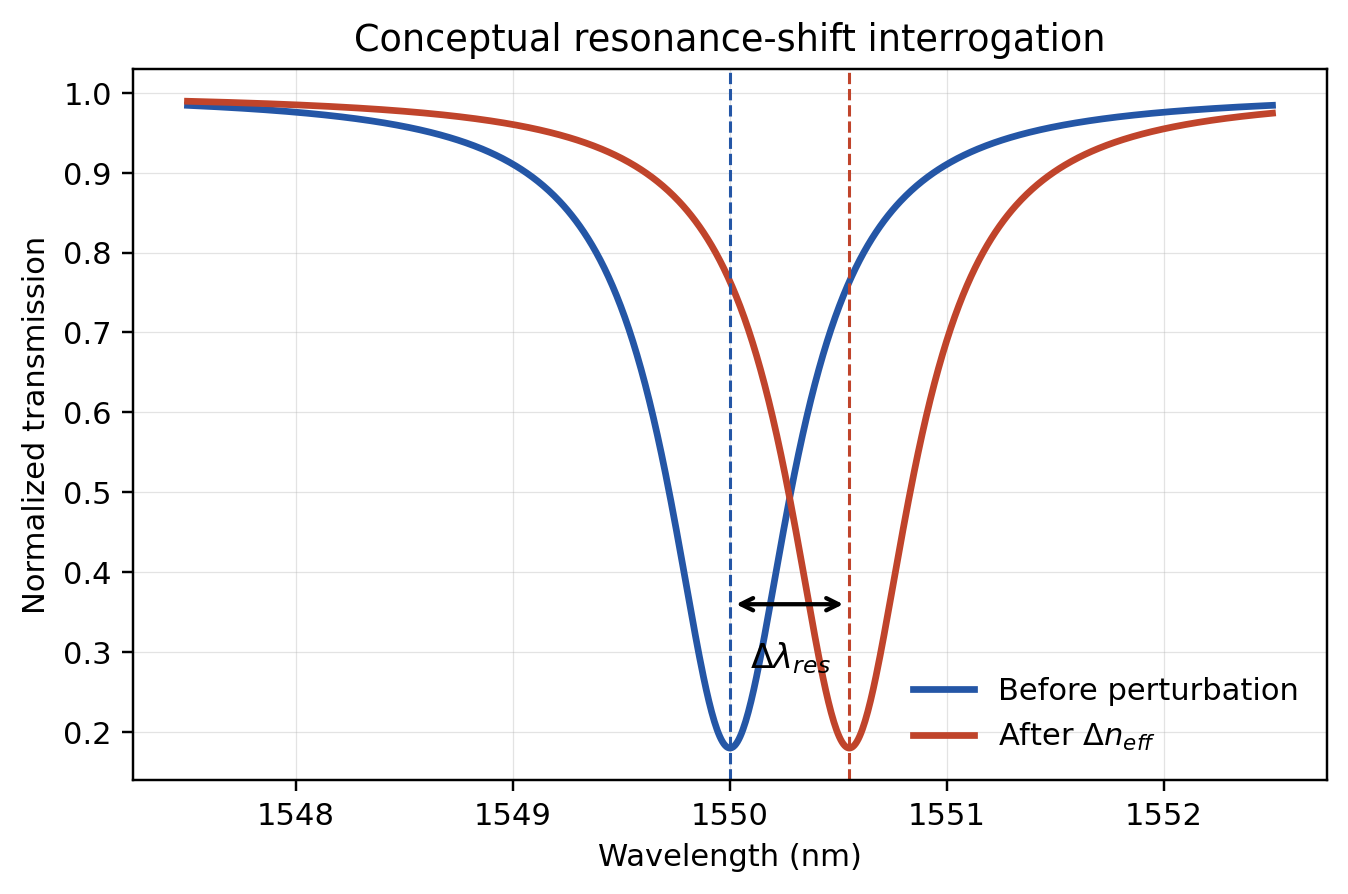
\includegraphics[width=0.78\linewidth]{figures/interrogation_principle_schematic.png}
\caption{Conceptual spectral interrogation of a microring resonance. The plot illustrates the expected direction of a resonance shift under a change in \(n_{\mathrm{eff}}\); it is not a simulated spectrum.}
\label{fig:interrogation}
\end{figure}

\section{Microring Resonator Theory}
An add-drop microring contains two straight bus waveguides and a ring waveguide, as shown in Fig.~\ref{fig:ring-schematic}. Light is coupled into the ring through evanescent coupling. At resonance, constructive interference builds the circulating field, producing a drop-port response and a through-port notch.

\begin{figure}[H]
\centering
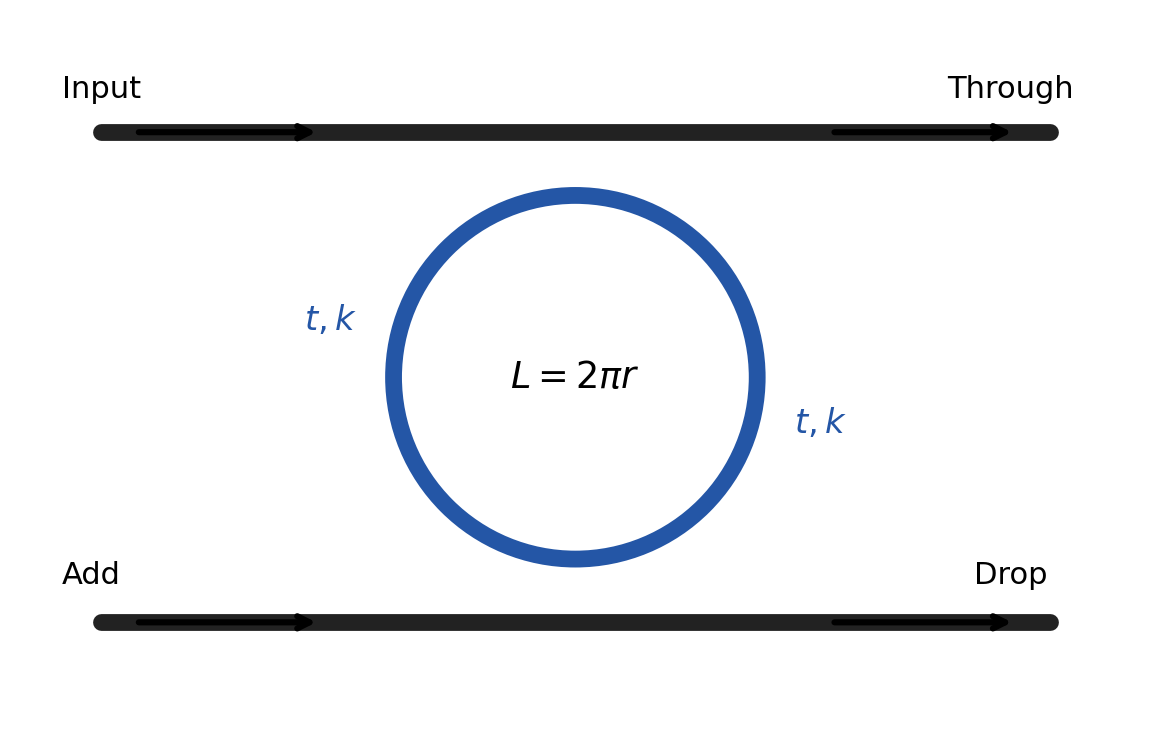
\includegraphics[width=0.76\linewidth]{figures/microring_add_drop_schematic.png}
\caption{Conceptual add-drop microring resonator. The field coupling coefficients are represented by through amplitude \(t\) and cross-coupling amplitude \(k\).}
\label{fig:ring-schematic}
\end{figure}

The resonance condition is
\begin{equation}
N \lambda_{\mathrm{res}} = 2 \pi r n_{\mathrm{eff}},
\label{eq:resonance}
\end{equation}
where \(N\) is the resonance order, \(r\) is the ring radius, and \(n_{\mathrm{eff}}\) is the effective index. The round-trip length is
\begin{equation}
L = 2 \pi r.
\label{eq:length}
\end{equation}

The wavelength-domain FSR is
\begin{equation}
FSR_\lambda = \frac{\lambda_{\mathrm{res}}^2}{n_g L},
\label{eq:fsr}
\end{equation}
with group index
\begin{equation}
n_g = n_{\mathrm{eff}} - \lambda \frac{d n_{\mathrm{eff}}}{d\lambda}.
\label{eq:group-index}
\end{equation}
Rearranging Eq.~\eqref{eq:fsr} gives
\begin{equation}
L = \frac{\lambda_{\mathrm{res}}^2}{n_g FSR_\lambda},
\qquad
r = \frac{L}{2\pi}.
\label{eq:ring-design}
\end{equation}

The quality factor and finesse are
\begin{equation}
Q = \frac{\lambda_{\mathrm{res}}}{FWHM},
\label{eq:q}
\end{equation}
\begin{equation}
\mathcal{F} = \frac{FSR}{FWHM}.
\label{eq:finesse}
\end{equation}

The coupling amplitudes obey
\begin{equation}
|t|^2 + |k|^2 = 1.
\label{eq:tk}
\end{equation}
Using the target \(Q\)-based relation supplied in the lab workflow,
\begin{equation}
|t| =
\sqrt{1+\left(\frac{n_g L \pi}{2Q\lambda}\right)^2}
-
\frac{n_g L \pi}{2Q\lambda}.
\label{eq:t-target}
\end{equation}
The coupling length is then
\begin{equation}
L_c =
\frac{\lambda_{\mathrm{res}}}{\pi \Delta n}
\sin^{-1}(|k|),
\label{eq:lc}
\end{equation}
where
\begin{equation}
\Delta n =
|n_{\mathrm{eff,sym}} - n_{\mathrm{eff,anti}}|.
\label{eq:delta-n}
\end{equation}
The coupled-mode index difference in Eq.~\eqref{eq:delta-n} must come from an FDE coupled-mode calculation; it is not available from the present files.

\section{INTERCONNECT System-Level Modelling}
The INTERCONNECT model represents the ring at circuit level using straight waveguides, waveguide couplers, a ring round-trip path, input/through/drop ports, and an optical network analyser. This level is useful for quickly predicting resonant transfer functions and checking how \(n_g\), round-trip length, and coupling coefficients affect FSR, linewidth, \(Q\), finesse, and drop-port power \cite{labmanual}.

\begin{figure}[H]
\centering
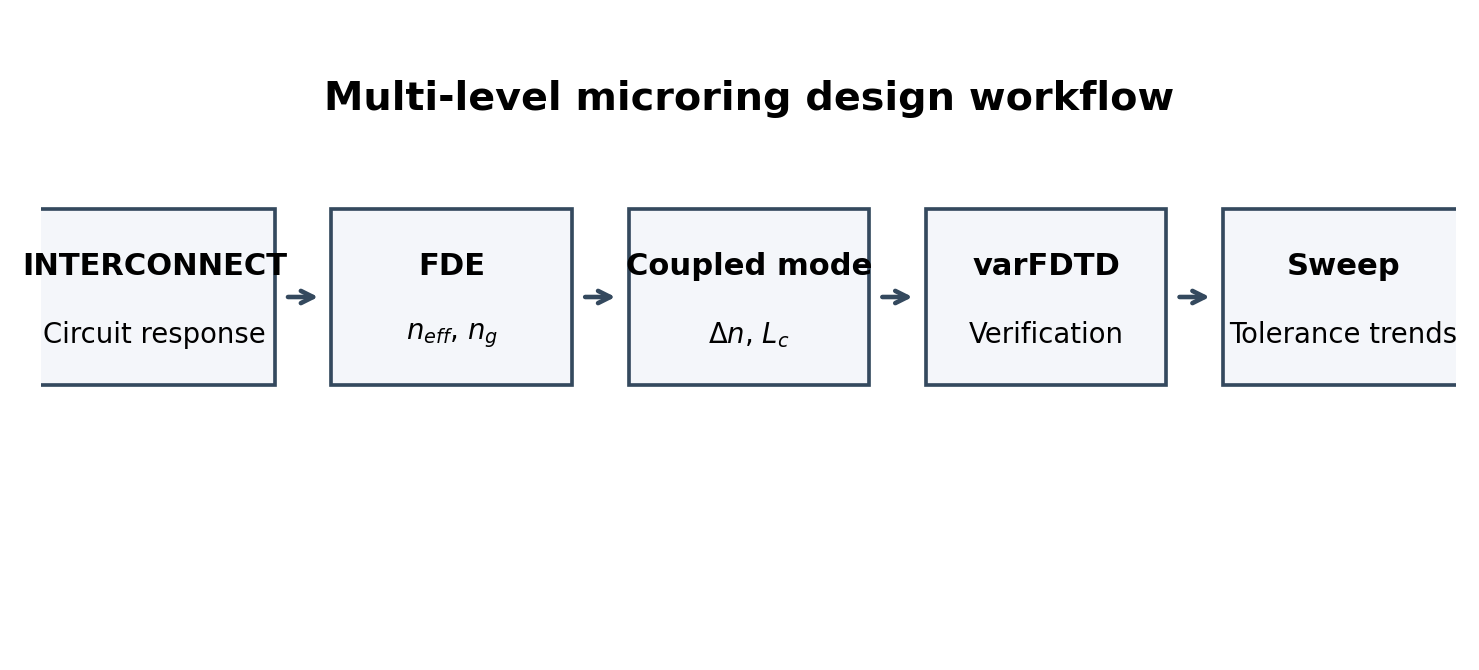
\includegraphics[width=0.92\linewidth]{figures/multilevel_workflow.png}
\caption{Conceptual multi-level workflow used for the report: system-level INTERCONNECT modelling, FDE modal extraction, coupled-mode design, varFDTD verification, and parameter sweeps.}
\label{fig:workflow}
\end{figure}

The original INTERCONNECT file \path{models_original/ring_resonator_student.icp} is available in the project directory but is not included in the Overleaf zip, following the requirement to avoid large Lumerical model files. No exported INTERCONNECT spectra or peak tables were found in \path{results/} or \path{figures/}. Therefore, Fig.~\ref{fig:workflow} is included only as a workflow schematic, not as a replacement for missing transfer functions.

\begin{table}[H]
\centering
\caption{INTERCONNECT quantities requested by the lab workflow. Missing entries should be filled after exporting ONA results from INTERCONNECT.}
\label{tab:interconnect-results}
\begin{tabular}{lll}
\toprule
Quantity & Value & Status \\
\midrule
Through-port transfer function & TODO & Not available from current simulation output \\
Drop-port transfer function & TODO & Not available from current simulation output \\
Resonance wavelength & TODO & Not available from current simulation output \\
FSR & TODO & Not available from current simulation output \\
FWHM & TODO & Not available from current simulation output \\
Drop-port \(Q\) factor & TODO & Not available from current simulation output \\
Drop-port finesse & TODO & Not available from current simulation output \\
Coupling coefficient & TODO & Not available from current simulation output \\
\bottomrule
\end{tabular}
\end{table}

\section{FDE Device-Level Mode Analysis}
The FDE stage resolves the waveguide cross-section and extracts the modal effective index and group index. The target SOI geometry is a silicon core of width \SI{400}{\nano\metre} and height \SI{200}{\nano\metre} on silicon dioxide, as shown in Fig.~\ref{fig:soi-cross-section}. The intended operating mode is the fundamental TE-like mode. A correct FDE study should verify the material mesh, boundary conditions, modal confinement, \(n_{\mathrm{eff}}\), and \(n_g\) near \SI{1550}{\nano\metre}.

\begin{figure}[H]
\centering
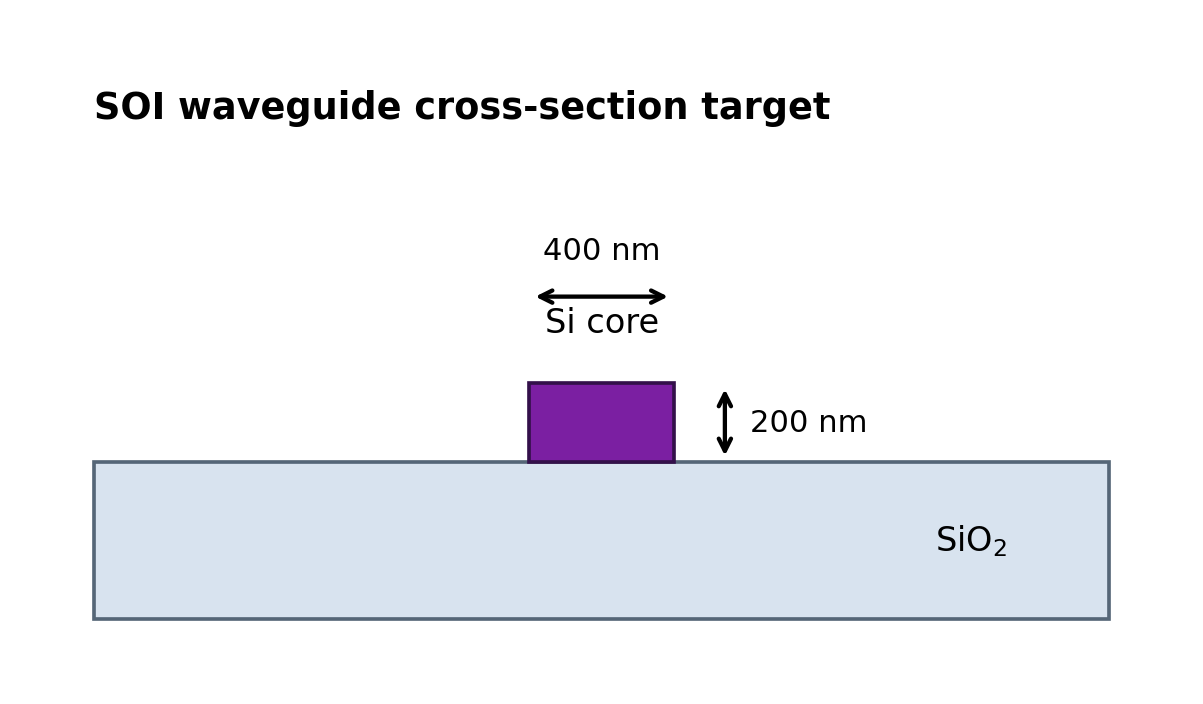
\includegraphics[width=0.72\linewidth]{figures/soi_cross_section_schematic.png}
\caption{Target SOI waveguide cross-section used for the FDE design stage. This schematic is based on the design target and is not an FDE mesh image.}
\label{fig:soi-cross-section}
\end{figure}

No FDE-exported mode profile, effective-index table, group-index table, or mesh image was present in the available \path{results/} or \path{figures/} directories. The original Lumerical MODE file \path{models_original/ring_resonator_studentv2_fde.lms} is available locally but was not modified or included in the Overleaf package.

Using Eq.~\eqref{eq:ring-design}, the ring length required for the target FSR can be written in terms of the unavailable FDE group index:
\begin{equation}
L = \frac{(\SI{1.55}{\micro\metre})^2}{n_g(\SI{0.0262}{\micro\metre})}
  = \frac{\SI{91.70}{\micro\metre}}{n_g},
\end{equation}
\begin{equation}
r = \frac{L}{2\pi}
  = \frac{\SI{14.59}{\micro\metre}}{n_g}.
\end{equation}
These expressions should be evaluated after extracting \(n_g\) at \SI{1550}{\nano\metre} from FDE. A numerical radius is not reported here because no real \(n_g\) value was available.

\begin{table}[H]
\centering
\caption{FDE outputs required for final design completion.}
\label{tab:fde-results}
\begin{tabular}{lll}
\toprule
Quantity & Value & Status \\
\midrule
\(n_{\mathrm{eff}}\) at \SI{1550}{\nano\metre} & TODO & Not available from current simulation output \\
\(n_g\) at \SI{1550}{\nano\metre} & TODO & Not available from current simulation output \\
TE mode confinement & TODO & Not available from current simulation output \\
Boundary condition check & TODO & Not available from current simulation output \\
Ring round-trip length \(L\) & \(\SI{91.70}{\micro\metre}/n_g\) & Target-derived expression \\
Ring radius \(r\) & \(\SI{14.59}{\micro\metre}/n_g\) & Target-derived expression \\
\bottomrule
\end{tabular}
\end{table}

\section{Coupling Design}
The coupling design converts target linewidth and power-transfer behaviour into a directional-coupler geometry. Physically, a smaller bus-ring gap increases evanescent overlap and therefore increases \(|k|\); a larger gap weakens coupling, increases \(|t|\), narrows the linewidth, and may increase \(Q\) and finesse at the cost of lower drop-port efficiency.

Using the target values \(\lambda_{\mathrm{res}}=\SI{1.55}{\micro\metre}\), \(FSR=\SI{0.0262}{\micro\metre}\), and \(Q=1800\), Eq.~\eqref{eq:t-target} can be evaluated after substituting \(L=\lambda^2/(n_g FSR)\), which cancels \(n_g\) in this target-only estimate. This gives
\begin{equation}
|t|_{\mathrm{target}} = 0.9497,\qquad
|k|_{\mathrm{target}} = 0.3131,\qquad
|k|_{\mathrm{target}}^2 = 0.0981.
\end{equation}
These are target-derived coupling estimates, not extracted Lumerical simulation results.

The actual physical coupling length requires
\(\Delta n = |n_{\mathrm{eff,sym}} - n_{\mathrm{eff,anti}}|\), obtained from an FDE simulation region containing both coupled waveguides. Since no coupled-mode export is available, \(L_c\) remains unavailable.

\begin{table}[H]
\centering
\caption{Coupling-design calculation status.}
\label{tab:coupling-results}
\begin{tabular}{lll}
\toprule
Quantity & Value & Provenance \\
\midrule
\(n_{\mathrm{eff,sym}}\) & TODO & Coupled FDE result not available \\
\(n_{\mathrm{eff,anti}}\) & TODO & Coupled FDE result not available \\
\(\Delta n\) & TODO & Requires coupled FDE result \\
\(|t|\) & 0.9497 & Target-based calculation, not simulated \\
\(|k|\) & 0.3131 & Target-based calculation, not simulated \\
\(|k|^2\) & 0.0981 & Target-based calculation, not simulated \\
\(L_c\) & TODO & Requires \(\Delta n\) from coupled FDE \\
\bottomrule
\end{tabular}
\end{table}

\section{varFDTD Verification}
varFDTD is a reduced 2.5D time-domain method that uses an effective-index approximation to collapse the 3D SOI geometry into a 2D propagation problem. It is less expensive than full 3D FDTD, while still providing broadband time-domain verification of the final microring layout \cite{labmanual}.

The intended verification outputs are the final device geometry, field profile, through/drop monitor spectra, and effective-index monitor data. The file \path{models_original/ring_resonator_studentv2_varfdtd.lms} is available locally, but no exported varFDTD field image, spectrum, or monitor data was found. Therefore, the comparison table below is structured for completion after simulation export.

\begin{table}[H]
\centering
\caption{Comparison of abstraction levels. Only target-derived expressions are filled; missing simulation outputs are marked explicitly.}
\label{tab:method-comparison}
\begin{tabular}{lllll}
\toprule
Method & Key input & FSR (nm) & \(Q\) & Finesse \\
\midrule
INTERCONNECT & Circuit parameters & TODO & TODO & TODO \\
FDE theory & \(n_g\) and radius & 26.2 target & N/A & N/A \\
varFDTD & Final device geometry & TODO & TODO & TODO \\
\bottomrule
\end{tabular}
\end{table}

After varFDTD completion, the most important checks are whether the drop-port spectrum reproduces the target FSR near \SI{26.2}{\nano\metre}, whether the resonance linewidth gives the intended \(Q\), and whether the field profile confirms that power is coupled into the ring and transferred to the drop port at resonance.

\section{Parameter Sweep}
The preferred open-ended analysis is a gap sweep over representative bus-ring gaps of \SI{80}{\nano\metre}, \SI{100}{\nano\metre}, \SI{120}{\nano\metre}, and \SI{150}{\nano\metre}. No numerical sweep data was found in \path{results/}, so the section is presented as a qualitative design discussion and a TODO table.

\begin{table}[H]
\centering
\caption{Gap sweep template. Numerical entries require exported FDE, INTERCONNECT, or varFDTD sweep data.}
\label{tab:gap-sweep}
\begin{tabular}{lllll}
\toprule
Gap (nm) & \(|k|^2\) & FSR (nm) & \(Q\) & Drop-port comment \\
\midrule
80 & TODO & TODO & TODO & Not available from current simulation output \\
100 & TODO & TODO & TODO & Not available from current simulation output \\
120 & TODO & TODO & TODO & Not available from current simulation output \\
150 & TODO & TODO & TODO & Not available from current simulation output \\
\bottomrule
\end{tabular}
\end{table}

The expected physical trend is that increasing the gap reduces evanescent coupling, so \(|k|\) decreases and \(|t|\) increases. Weaker coupling generally narrows the resonance linewidth and can increase \(Q\) and finesse, but it may also reduce drop-port efficiency and make the sensor response more sensitive to fabrication error and loss. Conversely, a smaller gap increases coupling and drop-port transfer but can broaden the resonance.

\section{Discussion}
FSR is a robust metric because it is mainly set by round-trip length and group index. Once the ring radius and waveguide dispersion are fixed, FSR changes smoothly and is less sensitive to small loss changes than linewidth-based metrics. In contrast, \(Q\) and finesse depend strongly on propagation loss, bend loss, coupling strength, spectral sampling resolution, mesh resolution, monitor placement, and numerical convergence. The lab notes explicitly caution that \(Q\) factor and finesse are sensitive to loss and minor numerical or fabrication variations \cite{labmanual}.

INTERCONNECT, FDE, and varFDTD represent different abstraction levels. INTERCONNECT is fast and circuit-oriented, making it useful for transfer functions and parameter sweeps. FDE resolves the waveguide cross-section and provides modal quantities such as \(n_{\mathrm{eff}}\), \(n_g\), and coupled-mode index splitting. varFDTD verifies the final geometry with a broadband propagation simulation under an effective-index approximation. Agreement among the three levels gives confidence; disagreement usually points to missing loss, dispersion, insufficient meshing, or an inconsistent coupling model.

For sensing, the resonator converts a measurand into a spectral shift. Analyte binding, refractive-index change, temperature, or strain modifies \(n_{\mathrm{eff}}\) or the optical path length. Practical interrogation can use wavelength scanning for direct spectra, resonance tracking for high resolution, or fixed-wavelength intensity readout for compact instrumentation. The fixed-wavelength approach is efficient but more vulnerable to laser power fluctuation unless differential through/drop readout or amplitude-comparison techniques are used.

Fabrication tolerance is critical. A small error in waveguide width or height changes dispersion and therefore \(n_g\), shifting the FSR and resonance locations. Gap variation changes \(|k|^2\), linewidth, extinction ratio, and drop efficiency. Sidewall roughness and bend loss reduce \(Q\), while minimum lithographic gap rules may constrain the strongest practical coupling. A complete design should therefore include mesh refinement, a gap and width tolerance sweep, and experimental calibration.

The available targets also contain a useful consistency check. The target \(Q=1800\) at \SI{1550}{\nano\metre} implies \(FWHM=\lambda/Q=\SI{0.861}{\nano\metre}\). The target finesse of 26 with \(FSR=\SI{26.2}{\nano\metre}\) implies \(FWHM=FSR/\mathcal{F}=\SI{1.008}{\nano\metre}\). These are close in scale but not identical, so the final design should specify whether the \(Q\) target or finesse target is prioritised after real spectra are exported.

\section{Conclusion}
This report package establishes an Overleaf-ready framework for the ELEC5516 Lab 5 SOI microring resonator sensor. The intended design uses a \SI{400}{\nano\metre} by \SI{200}{\nano\metre} SOI waveguide near \SI{1550}{\nano\metre}, targeting an FSR of \SI{26.2}{\nano\metre}, drop-port \(Q\) near 1800, and finesse near 26. The theory and workflow sections are complete, and the target-based expressions for ring length, radius, and coupling amplitudes are included with clear provenance.

The design cannot yet be claimed to meet the FSR, \(Q\), or finesse targets because no exported simulation results were available in \path{results/} or \path{figures/}. The next work is to run INTERCONNECT, extract FDE \(n_{\mathrm{eff}}\), \(n_g\), and coupled-mode indices, verify the final geometry with varFDTD, and complete a gap sweep. Future improvements should include mesh refinement, full 3D FDTD comparison, Monte Carlo fabrication-tolerance analysis, and experimental calibration.

\appendix
\section{Generated Files and Provenance}
This appendix summarises the files generated for the Overleaf package and records which numerical values are design targets, target-derived calculations, or missing simulation outputs.

\begin{table}[H]
\centering
\caption{Generated figure files included in the Overleaf project.}
\label{tab:generated-figures}
\small
\begin{tabular}{p{0.48\linewidth}p{0.44\linewidth}}
\toprule
Figure file & Role \\
\midrule
\path{figures/interrogation_principle_schematic.png} & Conceptual resonance-shift interrogation \\
\path{figures/microring_add_drop_schematic.png} & Conceptual add-drop microring layout \\
\path{figures/soi_cross_section_schematic.png} & Target SOI cross-section schematic \\
\path{figures/multilevel_workflow.png} & Multi-level design workflow schematic \\
\bottomrule
\end{tabular}
\end{table}

\begin{table}[H]
\centering
\caption{Raw/provenance data files included in the Overleaf project.}
\label{tab:data-files}
\small
\begin{tabular}{p{0.48\linewidth}p{0.44\linewidth}}
\toprule
Data file & Content \\
\midrule
\path{data/source_inventory.csv} & Source PDF inventory and page counts \\
\path{data/model_inventory.csv} & Local Lumerical model inventory, not included as models \\
\path{data/available_outputs_inventory.csv} & Inventory of available result/figure/script/work files \\
\path{data/target_calculations.csv} & Design targets and formula-derived values \\
\path{data/todo_items.csv} & Missing simulation outputs and reasons \\
\bottomrule
\end{tabular}
\end{table}

\begin{table}[H]
\centering
\caption{Calculation provenance summary.}
\label{tab:calculation-provenance}
\begin{tabular}{lll}
\toprule
Quantity & Value & Provenance \\
\midrule
\(\lambda_{\mathrm{res}}\) & \SI{1550}{\nano\metre} & Design target \\
\(FSR\) & \SI{26.2}{\nano\metre} & Design target \\
\(Q\) & 1800 & Design target \\
\(\mathcal{F}\) & 26 & Design target \\
\(FWHM\) from \(Q\) & \SI{0.861}{\nano\metre} & \(\lambda/Q\), target-derived \\
\(FWHM\) from finesse & \SI{1.008}{\nano\metre} & \(FSR/\mathcal{F}\), target-derived \\
\(L\) & \(\SI{91.70}{\micro\metre}/n_g\) & Requires FDE \(n_g\) \\
\(r\) & \(\SI{14.59}{\micro\metre}/n_g\) & Requires FDE \(n_g\) \\
\(|t|\), \(|k|\), \(|k|^2\) & 0.9497, 0.3131, 0.0981 & Target-based only \\
\(\Delta n\), \(L_c\) & TODO & Requires coupled FDE \\
\bottomrule
\end{tabular}
\end{table}

The script used to create the package is \path{scripts/generate_report_package.py}. It generated the project structure, provenance CSV files, conceptual figures, LaTeX section files, and README. It did not modify \path{models_original/}.


\bibliographystyle{unsrt}
\bibliography{references}

\end{document}
